\subsection{Одноклассовый метод опорных векторов, One-Class SVM}

One-Class Support Vector Machine (One-Class SVM или просто One-SVM) представляет собой одноклассовый неконтролируемый метод обнаружения аномалий \cite{Skilear-One-Class-SVM-Doc}. Основной идеей One-SVM является установление границы, охватывающей области с высокой плотностью данных, при этом исключая заданную долю данных $\nu = (0;\ 1]$ (гиперпараметр модели), которая (по мнению пользователя модели) представляет собой верхнюю границу числа аномалий в данных (см. рисунок \ref{fig:one-class-svm}).

\begin{figure}
  \centering
  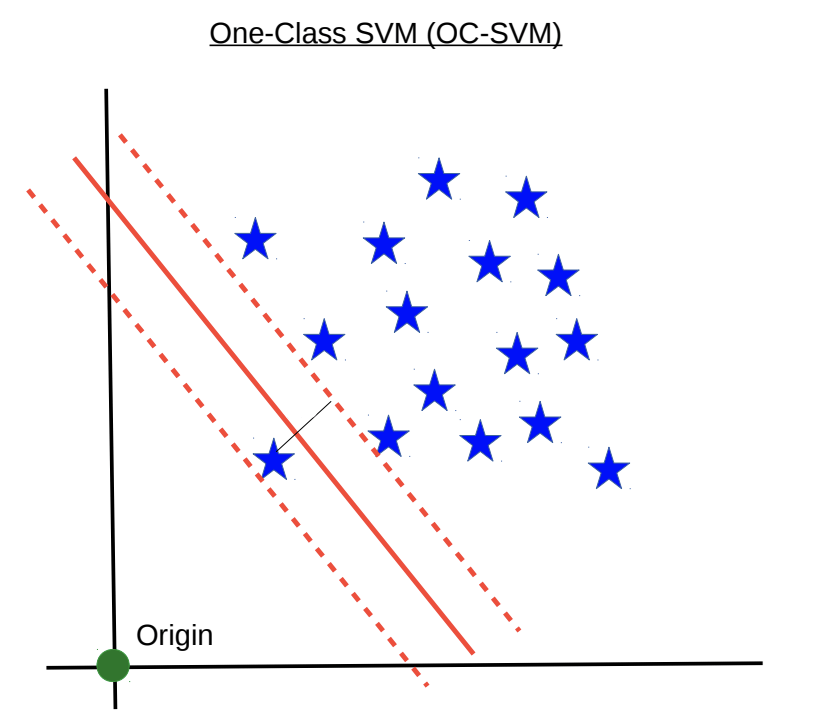
\includegraphics[scale=0.5]{inc/images/one-class-svm.png}
  \caption{Специализация метода опорных векторов для поиска выбросов \cite{SVM-Lecture}}
  \label{fig:one-class-svm}
\end{figure}

Главной целью One-SVM является поиск гиперплоскости, разделяющей данные от источника (начала координат). Для достижения этой цели метод использует линейный классификатор, но с использованием ядра --- функции, которая отображает пространство признаков в пространство высшей размерности. Канонично данный kernel trick \cite{Anomaly-Detection-One-Class-SVM} позволяет разделять классы, линейно неразделимые в текущем признаковом пространстве (см. рисунок \ref{fig:nonlinear-separation-demo}). Таким образом на выходе получается модель с нелинейными границами в исходном пространстве переменных задачи.

\newpage

RBF (Radial Basis Function) \cite{RBF-Kernel-in-SVM} часто является наиболее широко применяемым ядром для One-SVM ввиду нелинейности и гибкой адаптации к различным распределениям данных. Данное ядро определяется функцией (\ref{RBF_def}):

\begin{equation}\label{RBF_def}
    K_{RBF}(\overline{x},\ \overline{x}') = e^{-\gamma \lVert \overline{x} - \overline{x}' \rVert^2},
\end{equation}
где $\overline{x},\ \overline{x}' \in \mathbb{R}^k$ --- выборки, векторы в входном пространстве размерности $k$, \\
$\gamma$ --- свободный параметр, который позволяет настраивать влияние соседних точек на границу принятия решения.

\begin{figure}
  \centering
  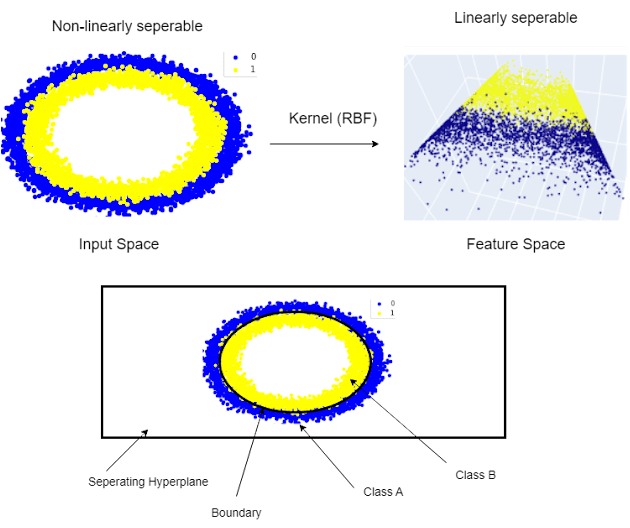
\includegraphics[scale=0.45]{inc/images/nonlinear-separation-demo.png}
  \caption{Нелинейное разделение данных на основе пороговой гиперплоскости в пространстве признаков \cite{RBF-Kernel-in-SVM}}
  \label{fig:nonlinear-separation-demo}
\end{figure}

Таким образом, в результате обучения One-Class SVM стремится создать гиперплоскость, которая наилучшим образом ограничит область с высокой плотностью данных (см. рисунок \ref{fig:rbf-demo}), считая все остальные области аномальными. Этот метод демонстрирует свою эффективность в выявлении аномалий и обеспечивает контроль над тем, какая доля данных считается аномальной, благодаря гиперпараметру $\nu$.

\begin{figure}
  \centering
  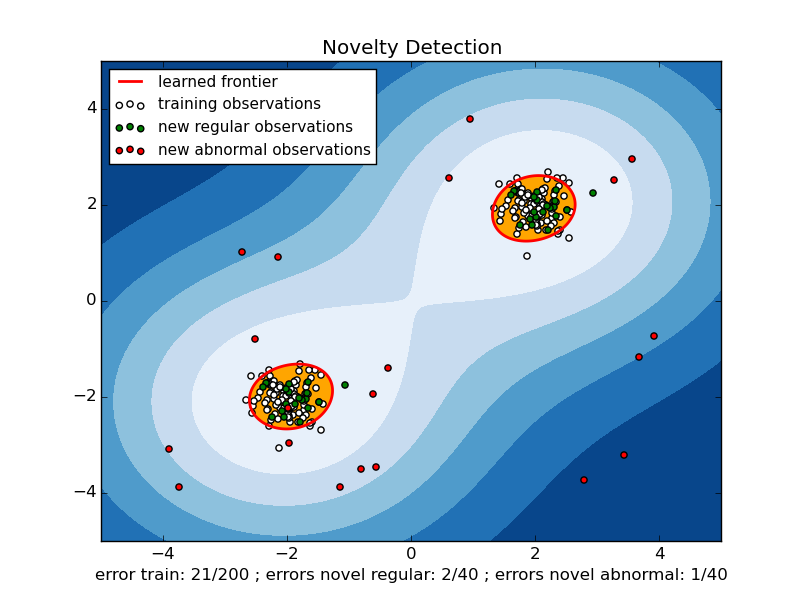
\includegraphics[scale=0.3]{inc/images/rbf-demo.png}
  \caption{Пример обнаружения аномалий на основе One-SVM с нелинейным ядром RBF \cite{Skilear-RBF-Doc}}
  \label{fig:rbf-demo}
\end{figure}

% При использовании One-Class SVM функция принятия решения решений можно формализовать соотношением (\ref{f_ocsvm}).
% \begin{equation}\label{f_ocsvm}
%     f(\overline{x_i}) = sign\Big[K(\overline{x_i},\ \overline{x_j}) - b\Big],
% \end{equation}
% где $K$ --- функция ядра (может быть определена, как в формуле (\ref{RBF_def})), \\
% $\overline{w}$ --- весовые коэффициенты, корректирующиеся в процессе обучения модели, \\
% $b$ --- пороговое значение смещения, которое задаёт сдвиг гиперплоскости относительно начала координат.

% Ключевой гиперпараметр $\nu \in (0,\ 1]$ задаёт максимальную допустимую долю аномальных экземпляров в данных, что позволяет установить ограничение на вероятность ложноположительного срабатывания:
% \begin{equation}\label{alpha_ocsvm}
%     \alpha = P\Big\{ f(\overline{x_i}) = 1\ \Big|\ t_i\ -\ \text{«нормальный» экземпляр} \Big\} \leq p,
% \end{equation}
% где, при корректном выборе $\nu$, порог $p$ (например, $0,05$) выполняется.

% При этом модель стремится инкапсулировать область с высокой плотностью нормальных данных, минимизируя вероятность ошибки II-го рода, которая определяется как
% \begin{equation}\label{beta_ocsvm}
%     \beta = P\Big\{ f(\overline{x_i}) = -1\ \Big|\ t_i\ -\ \text{«аномальный» экземпляр} \Big\}.
% \end{equation}

Оптимизация модели One-Class SVM направлена на минимизацию $\beta$ при условии, что вероятность ложноположительного срабатывания $\alpha$ не превышает установленный порог $p$. Применение нелинейного ядра (например, RBF), позволяет отобразить исходное пространство признаков в пространство более высокой размерности, что способствует построению адаптивной и нелинейной границы принятия решения, способной учитывать сложную структуру сетевого трафика. Это непосредственно соответствует цели оптимизации, сформулированной в (\ref{task_formulation}).
